% !TeX program = lualatex
% GraphIV pitch: 20 minutes of talking, then a live demo and questions.
% Build with `latexmk graphiv.tex`, which runs lualatex per the template's latexmkrc.
\documentclass[aspectratio=169, 11pt]{beamer}

\usetheme[palette=Natsumikan, variant=dark]{kuroma}

\usepackage{booktabs}

% Emphasis carries colour, not weight alone. Titles are already primary, so bold takes
% tertiary and italic secondary, since both oranges read as one colour.
\let\oldtextbf\textbf
\renewcommand{\textbf}[1]{{\color{ktertiary}\oldtextbf{#1}}}
\let\oldemph\emph
\renewcommand{\emph}[1]{{\color{ksecondary}\oldemph{#1}}}
\usepackage{tikz}
\usetikzlibrary{arrows.meta, positioning, fit, backgrounds}

\title{GraphIV}
\subtitle{Knowledge graph driven deep research tool}
\author{KK Thuwajit}
\institute{\texttt{kuroma.dev}}
\date{}

\begin{document}

\begin{frame}[plain, noframenumbering, c]
  \titlepage
\end{frame}

\begin{frame}{Running order}
  \tableofcontents[hideallsubsections]
\end{frame}

% ===================================================================
\section{Motivation}

\begin{frame}{Research Question}
  A question I have at the start of projects:
  \begin{kbox}{}
    \begin{center}
      \Large
      \emph{What are people doing in (field) right now?}\\[0.4em]
      \emph{And what led them to doing it?}
    \end{center}
  \end{kbox}
  \medskip
  Is actually two questions in one:
  \begin{itemize}
    \item The \textbf{frontier} half wants what is recent and relevant.
    \item The \textbf{lineage} half wants the chain that leads to the frontier.
  \end{itemize}
  \medskip
  {\small A list of papers answers neither!}
\end{frame}

\begin{frame}{Available Tools}
  \begin{columns}[T]
    \begin{column}{0.32\textwidth}
      \begin{kbox}[equal height group=tools]{AI search}
        One web search, retrieve whatever comes back, answer over it.
        
        \textbf{Shallow}: As deep as whatever comes first
      \end{kbox}
    \end{column}
    \begin{column}{0.32\textwidth}
      \begin{kbox}[equal height group=tools]{Deep research}
        Gemini, Claude, ChatGPT deep search that finds papers on its own.
        
        \textbf{No lineage}: Finds papers. Cannot say which descends from which.
      \end{kbox}
    \end{column}
    \begin{column}{0.32\textwidth}
      \begin{kbox}[equal height group=tools]{Consensus}
        The closest thing. Built to answer \emph{what is the consensus in an area}.

        \textbf{Different question}: Aggregates agreement, not development.
      \end{kbox}
    \end{column}
  \end{columns}

  \textbf{The gap}: all three treat papers as independent sources. The citations/lineages that connects them gets neglected.
\end{frame}

\begin{frame}{Goals}
  \begin{enumerate}
    \item A tool that finds what people are doing now and \emph{why} they are doing it given any research question
    \item Local, self-hostable, open, and reliable. One consumer machine, local database, and every claim traceable.
    \item A generalizable technique and findings.
  \end{enumerate}

  \textbf{Claim:} Citations link related papers together. Knowing \textbf{why} $A$ cites $B$ explains the development in that field.

  Graph retrieval is active: GraphRAG builds a graph over a corpus with an
  LLM~\cite{graphrag_local_global}; G-Retriever answers over one textual
  graph~\cite{gretriever}; PaSa is an agent that follows citations~\cite{pasa}.

  \textbf{None fit here}: the first cannot scale to 3.1M papers, the second targets a node's
  attributes, the third needs an API call per hop.

\end{frame}

% ===================================================================
\section{Method}

\begin{frame}{The Corpus}
  \begin{columns}[T]
    \begin{column}{0.5\textwidth}
      \begin{kbox}[equal height group=cA]{Papers}
        3{,}073{,}288 arXiv papers, PDF and LaTeXML HTML on disk.
      \end{kbox}
      \begin{kbox}[equal height group=cB]{Citations}
        176{,}934{,}085 occurrences parsed from HTML bodies.

        36{,}688{,}723 distinct in-corpus edges.
      \end{kbox}
    \end{column}
    \begin{column}{0.5\textwidth}
      \begin{kbox}[equal height group=cA]{Intent, per edge}
        background \textbar\ uses \textbar\ extends \textbar\ compares \textbar\ critiques \textbar\ motivates
      \end{kbox}
      \begin{kbox}[equal height group=cB]{Embeddings}
        3.10M vectors, nomic-embed-text-v2-moe~\cite{nomic}, pgvector HNSW.

        \textbf{Stock weights}: nothing here is fine-tuned.
      \end{kbox}
    \end{column}
  \end{columns}
\end{frame}

\begin{frame}{Corpus Shape}
  \begin{columns}[T]
    \begin{column}{0.5\textwidth}
      \includegraphics[width=\linewidth, height=0.45\textheight, keepaspectratio]{figures/indegree_loglog.png}
    \end{column}
    \begin{column}{0.5\textwidth}
      \includegraphics[width=\linewidth, height=0.45\textheight, keepaspectratio]{figures/per_year.png}
    \end{column}
  \end{columns}
  \medskip
  \textbf{The tail is the problem}: ResNet is cited 117,137 times inside the corpus,
  BERT 85,284, Attention 80,414. Rank on citation count and you return those for every question.
\end{frame}

\begin{frame}{Edge Labels}
  \begin{columns}[T]
    \begin{column}{0.52\textwidth}
      \includegraphics[width=\linewidth, height=0.5\textheight, keepaspectratio]{figures/intent_mix.png}
    \end{column}
    \begin{column}{0.44\textwidth}
      \begin{kbox}{Student, held out ($n{=}13{,}521$)}
        intent accuracy 0.844

        intent macro-F1 0.723

        polarity accuracy 0.947
      \end{kbox}
      A Gemma teacher labels a sample, a DistilBERT student labels all 177M.
    \end{column}
  \end{columns}
  \medskip
  \textbf{Weak classes}: \emph{uses} against \emph{extends}, which are genuinely close in an
  author's phrasing.
\end{frame}

\begin{frame}{Pipeline}
  \begin{center}
  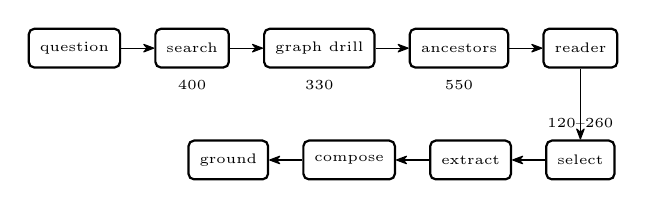
\begin{tikzpicture}[
      node distance=0.38cm and 0.42cm, >={Stealth[round]},
      stage/.style={draw, rounded corners=2pt, align=center, font=\tiny,
                    minimum height=1.4em, inner xsep=4pt, thick},
      lbl/.style={font=\tiny, align=center}]
    \node[stage] (q)   {question};
    \node[stage, right=of q]  (pool) {search};
    \node[stage, right=of pool] (drill) {graph drill};
    \node[stage, right=of drill] (anc) {ancestors};
    \node[stage, right=of anc] (grade) {reader};
    \node[stage, below=0.9cm of grade] (sel) {select};
    \node[stage, left=of sel] (ext) {extract};
    \node[stage, left=of ext] (comp) {compose};
    \node[stage, left=of comp] (gr) {ground};
    \draw[->] (q)--(pool); \draw[->] (pool)--(drill); \draw[->] (drill)--(anc);
    \draw[->] (anc)--(grade); \draw[->] (grade)--(sel); \draw[->] (sel)--(ext);
    \draw[->] (ext)--(comp); \draw[->] (comp)--(gr);
    \node[lbl, below=0.03cm of pool] {400};
    \node[lbl, below=0.03cm of drill] {330};
    \node[lbl, below=0.03cm of anc] {550};
    \node[lbl, above=0.03cm of sel] {120--260};
  \end{tikzpicture}
  \end{center}
  \medskip
  \textbf{Search only opens the shortlist.} A vector search over abstracts gets 400 papers in.
  The drill then \emph{cuts} to 330, and citations add the most: roughly a hundred papers a
  question arrive through the graph and are never found by search.
\end{frame}

\begin{frame}{LeyLine}
  A \textbf{magnet} is a paper the reader rated highly. A walk starts where the most magnet mass
  is reachable and follows citations \emph{forward}, cited to citing.
  \begin{kbox}{}
  {\scriptsize\ttfamily
  adj $\leftarrow$ reverse(edges)\\
  w $\leftarrow$ \{magnet: 1\}\\
  repeat MAX\_LINEAGES:\\
  \hspace*{1.2em} root $\leftarrow$ argmax reachable\_mass(adj, w)\\
  \hspace*{1.2em} thread $\leftarrow$ walk(root, k=1)\\
  \hspace*{1.2em} collect magnets on thread; w[collected] *= GAMMA\\
  return papers by collection frequency over SEEDS runs
  }
  \end{kbox}
  \textbf{k=1} makes a line, not a bush. \textbf{GAMMA} decay makes the next walk find a
  different story. It spends 8 of the landmark slots.
\end{frame}

\begin{frame}{Joint Retrieval Method}
  The two signals, spent as one budget of 80 slots.
  \begin{kbox}{}
  {\scriptsize\ttfamily
  graph  $\leftarrow$ citations per year, as a percentile within the pool\\
  reader $\leftarrow$ relevance from $-2..2$, mapped onto 0..1\\
  score  $\leftarrow$ 0.65 $\times$ graph \ + \ 0.35 $\times$ reader\\
  take the top 72 by score, give the last 8 to LeyLine
  }
  \end{kbox}
  \textbf{Citations per year, not raw count}: a paper from last year with 200 citations beats a
  2015 hub with 2000. Age is what stops the same five famous papers answering every question.
  \medskip

  \textbf{A paper the reader rejects is dropped} from the ranking, but stays in the graph, since
  an off-topic paper can still be the link between two on-topic ones.
\end{frame}

\begin{frame}{Generation Loop}
  \begin{enumerate}
    \item \textbf{Grade}: the reader gives each candidate a role and a relevance in $-2..2$.
    \item \textbf{Select}: landmarks, by survey or frontier mode.
    \item \textbf{Extract}: a question-specific schema, filled per paper from full text.
    \item \textbf{Compose}: a node table plus an intent-grouped adjacency list, so the writer
          sees relationships and not just papers.
    \item \textbf{Judge}: a verdict decides whether to expand and retrieve again. It stops on its own.
    \item \textbf{Ground}: every cited id is corpus-verified, typos corrected, fabrications stripped.
  \end{enumerate}
  Steps 1 to 5 all run on one \textbf{Gemma-4-26B}, off the shelf, on the same 3090.
  \medskip

  \textbf{Step 6 is mechanical}, not a prompt. A report cannot cite a paper that does not exist.
\end{frame}

% ===================================================================
\section{Evaluation}

\begin{frame}{Survey-qrels}
  \begin{kbox}{The construction}
    Take a survey paper. \textbf{Hide it.} Freeze the corpus to its publication month. Have an
    LLM write the question it answers.

    The answer key is the survey's own reference list, filtered to works it discusses three or
    more times.
  \end{kbox}
  60 surveys, 2022--2024, 17 archives. 30 dev / 30 test, arms chosen on dev. 1,617 positive citations,
  860 reachable at all.
  \medskip
  \textbf{Why not a relevance judgement}: nobody labels 3.1M papers. A survey's author already
  did the labelling, for their own field, with care no annotator will match.
\end{frame}

\begin{frame}{LitSearch}
  \begin{columns}[T]
    \begin{column}{0.55\textwidth}
      \includegraphics[width=\linewidth, height=0.55\textheight, keepaspectratio]{figures/on_their_task.png}
    \end{column}
    \begin{column}{0.42\textwidth}
      597 queries~\cite{litsearch}. Published rows are their table 3; ours measured through
      their index.
      \begin{kbox}{Reader rerank}
        \textbf{75.8} specific R@5

        \textbf{74.7} broad R@20
      \end{kbox}
      Between GritLM-7B and GPT-4 reranking over it, on one 3090.
    \end{column}
  \end{columns}
  \medskip
  \textbf{The caveat}: LitSearch has 1.07 positive citations per query. It measures finding
  \emph{one} paper, so it validates components, not the claim.
\end{frame}

\begin{frame}{Support Check}
  \begin{kbox}{The measurement}
    Every citing sentence is checked against \emph{that paper's own text}, retrieving the
    passages nearest the claim. A sentence citing several papers passes if any one supports it.
  \end{kbox}
  \begin{kbox}{The control}
    Break citations on purpose: swap the cited id for the \textbf{most similar paper the same
    report cites}. Same topic, so vocabulary alone will not catch it.

    Then score the broken ones exactly like the real ones.
  \end{kbox}
  Two judge families, Gemma and Qwen. Gemma wrote the reports, so it is the one with a reason
  to flatter itself.
\end{frame}

% ===================================================================
\section{Results}

\begin{frame}{Positive Citations, by Stage}
  \begin{columns}[T]
    \begin{column}{0.5\textwidth}
      \includegraphics[width=\linewidth, height=0.5\textheight, keepaspectratio]{figures/by_stage.png}
    \end{column}
    \begin{column}{0.46\textwidth}
      Eleven levers, grouped by stage. Spread:
      \begin{kbox}{positive citations moved, of 1{,}617}
        vector channel \hfill 20

        lexical channel \hfill 14

        \textbf{citation graph} \hfill \textbf{96}
      \end{kbox}
    \end{column}
  \end{columns}
  \medskip
  \textbf{The ceiling is set before ranking.} 757 of 1,617 never reach the pool at all.
\end{frame}

\begin{frame}{Two Ways to Spot a Paper}
  \begin{columns}[T]
    \begin{column}{0.46\textwidth}
      \includegraphics[width=\linewidth, height=0.5\textheight, keepaspectratio]{figures/complementarity.png}
    \end{column}
    \begin{column}{0.5\textwidth}
      How the field cites it, or how a model reads it. Both beat chance by the same amount:
      \begin{kbox}{lift over base rate}
        citations per year \hfill 2.89

        reader relevance \hfill 2.88

        text similarity \hfill 1.93
      \end{kbox}
    \end{column}
  \end{columns}
  \medskip
  But they point at \emph{different} papers: 160 only the graph finds, 159 only the reader.
  \textbf{So use both.}
\end{frame}

\begin{frame}{With and Without the Graph}
  \begin{center}
    \begin{tabular}{lccc}
      \toprule
      digest & coverage & supported & broken caught \\
      \midrule
      graph      & 0.605 & \textbf{0.707} & 0.703 \\
      no graph   & 0.586 & \textbf{0.754} & 0.704 \\
      \bottomrule
    \end{tabular}
  \end{center}
  \medskip
  \textbf{The graph does not help here.} Same pool, same budget, edges 10,227 against 0.
  No-graph led in 8 of 10 matched pairs.
  \begin{kbox}{Untested hypothesis}
    Told \emph{A cites B}, a writer produces \emph{A builds on B}: true of the graph,
    unsupported by either paper.
  \end{kbox}
\end{frame}

\begin{frame}{How to Combine Them}
  \begin{center}
    \includegraphics[width=0.80\linewidth, height=0.70\textheight, keepaspectratio]{figures/selectors.png}
  \end{center}
\end{frame}

\begin{frame}{Finding Newer Work}
  \begin{columns}[T]
    \begin{column}{0.48\textwidth}
      \includegraphics[width=\linewidth, height=0.5\textheight, keepaspectratio]{figures/ceiling.png}
    \end{column}
    \begin{column}{0.48\textwidth}
      Of the papers LeyLine picks, how many did the survey actually cite?
      \begin{kbox}{picked papers that were cited by the survey}
        LeyLine \hfill \textbf{18.1\%}

        the slots it replaced \hfill 10.4\%

        picking at random \hfill 4.3\%
      \end{kbox}
      Median age \textbf{3 years}, against 7.
    \end{column}
  \end{columns}
  \textbf{Half the age, nearly twice as often right.} That is the \emph{what is happening now}
  half of the opening question.
\end{frame}

\begin{frame}{Citation Approval}
  \begin{columns}[T]
    \begin{column}{0.47\textwidth}
      \includegraphics[width=\linewidth, height=0.5\textheight, keepaspectratio]{figures/checker.png}
    \end{column}
    \begin{column}{0.49\textwidth}
      Ask a model: \emph{does this paper actually say that?}
      \begin{kbox}{approved, of 818 sentences}
        real citations \hfill \textbf{7 in 10}

        citations we broke \hfill \textbf{under 2 in 10}
      \end{kbox}
      Two model families, agreeing on 90.6\% of sentences.
    \end{column}
  \end{columns}
  \medskip
  \textbf{The second number is what makes the first one mean anything.} A checker that approves
  everything would score 10 in 10 on both.
\end{frame}

\begin{frame}{What a Run Costs}
  Five topics, one instruction template, effort 4, one RTX 3090.
  \begin{center}
    \begin{tabular}{lrrrr}
      \toprule
      topic & wall & cited & verified & 2026 \\
      \midrule
      neural audio codecs        & 6:03 & 45 & 45 & 11 \\
      test-time compute          & 2:46 & 56 & 56 & 5 \\
      state-space models         & 7:38 & 51 & 51 & 7 \\
      RL for theorem proving     & 5:14 & 60 & 60 & 12 \\
      QEC neural decoders        & 5:09 & 55 & 55 & 5 \\
      \midrule
      \textbf{total}             &      & \textbf{267} & \textbf{267} & \textbf{40} \\
      \bottomrule
    \end{tabular}
  \end{center}
  \textbf{267 of 267 ids verified, 0 fabricated}, and 97 papers from 2025 or later. Under eight
  minutes a question on one consumer GPU.
\end{frame}

% ===================================================================
\section{Discussion}

\begin{frame}{Findings}
  \begin{enumerate}
    \item \textbf{Retrieval is decided before ranking.} The pool stage moves 96 papers where
          the ranking rule moves 18.
    \item \textbf{The graph and a reading model are equally strong and largely disjoint.}
          2.89 against 2.88, with 160 papers only one sees and 159 only the other.
    \item \textbf{Walking citations forward finds young work that lasts.} 18.1\% against
          10.4\%, at a median age of 3 years against 7, using 8 slots of 80.
    \item \textbf{Grounding is mechanical, faithfulness is not.} Every cited id exists by
          construction. Whether the paper supports the sentence is seven in ten.
  \end{enumerate}
\end{frame}

\begin{frame}{Contributions}
  \begin{columns}[T]
    \begin{column}{0.48\textwidth}
      \begin{kbox}[equal height group=coA]{A dataset}
        Every arXiv paper and every citation between them, labelled with \emph{why} one paper
        cites another. 3.1M papers, 177M edges.
      \end{kbox}
      \begin{kbox}[equal height group=coB]{A retrieval method}
        LeyLine: walk citations forward from the papers a reader liked, and see where the
        threads land.
      \end{kbox}
    \end{column}
    \begin{column}{0.48\textwidth}
      \begin{kbox}[equal height group=coA]{An evaluation}
        Hide a survey, roll the corpus back to its month, ask its question, count how much of
        its reference list returns. 60 surveys, nobody labelled anything.
      \end{kbox}
      \begin{kbox}[equal height group=coB]{A composer}
        Turns the retrieved papers into a written review where every citation is checked against
        the corpus before it ships.
      \end{kbox}
    \end{column}
  \end{columns}
\end{frame}

\begin{frame}{Open Problems}
  \begin{kbox}{Forward impact}
    Every evaluation here is backward-looking. The question I want is whether a paper
    retrieved today \emph{becomes} important.

    Freeze at $T$, retrieve, label by citations accrued over two years, normalised against
    expected accrual, or it measures fame.
  \end{kbox}
  \begin{kbox}{The uncited half}
    818 of 1,372 sentences carry a citation. Whether the rest invent anything is not
    measurable by prompting: two schemes failed a second judge, the stricter at
    $\kappa = 0.003$. \textbf{It needs human labels.}
  \end{kbox}
\end{frame}

\begin{frame}[plain, noframenumbering, c]
  \begin{center}
    {\Huge Thank you}\\[1.2em]
    {\large Demo: \texttt{graphiv.kuroma.dev}}\\[0.6em]
  \end{center}
\end{frame}

\begin{frame}[allowframebreaks]{References}
  \bibliographystyle{plain}
  \bibliography{refs}
\end{frame}

\end{document}
